\section{Einleitung}
\subsection{Unternehmen}
guidelines: https://ilias.th-koeln.de/goto.php?target=file_1364683_download&client_id=ILIAS_FH_Koeln

beispiel simon kurth
https://inovex.sharepoint.com/sites/lab/Abgeschlossene%20Thesen/Forms/AllItems.aspx?id=%2Fsites%2Flab%2FAbgeschlossene%20Thesen%2FSimon%5FKurth%5FVergleich%5Fvon%5FKubernetes%5FNetzwerk%5FPlug%2DIns%5Ffuer%5Fden%5FPraxiseinsatz%2Epdf&parent=%2Fsites%2Flab%2FAbgeschlossene%20Thesen&p=true&originalPath=aHR0cHM6Ly9pbm92ZXguc2hhcmVwb2ludC5jb20vOmI6L3MvbGFiL0VWcF9DZFdLTm1wTW9kU2tVTHJ2bk1BQms3bWltSHRzTXRrMTk3Tkh4aU1kalE_cnRpbWU9TjlUd1VOZTcyRWc

- outline the work
problemdomäne
derzeitige situation
was ist das problem ?
wie löse ich dies ?
was gehört nicht zum scope ?
was sind die kern resultate
- abgrenzen von frameworks / tools / konzepte / methoden die ich benutze

eher eine management summary
2-3 seiten

2 ) domäne andwendungsfel

\section{Introduction}
\subsection{Company}
"Inovex is an IT project centre driven by innovation and quality, focusing its services on "Digital Transformation". The main three subdivisions are "Application Development", "Data Management \& Analytics" and "IT Engineering \& Operations" in which I work in the scope of this project.\\
"IT Engineering and Operations" handles the combined disciplines required for the flexible, reliable operation of systems in data centres: the design, installation and configuration of server infrastructures, and the daily maintenance and running of these systems. The focus is on high availability and scalability, migrations, the cloud, and open-source data centre management."\cite{inovex}

\subsubsection{Philosophy}
"Here at inovex, we are using an iterative strategy process to manage our own agile transformation. We also believe in flat hierarchies, and we base all our decisions on agile values.\\
As all our project teams are self-organised and agile skills are, therefore, essential, every new inovex employee receives training in agile methods. We also support our employees by holding meetings in agile formats (like Lean Coffee) and by facilitating the internal transfer of knowledge (through brown bag lunches and tech days, for example).\\
Many of our internal teams work agilely and thus enjoy a high level of transparency, quality and efficiency. Our Marketing Team, HR Team and Sales Team have each established different agile methods tailored specifically to their requirements and they use these in combination with our ISO-certified quality management processes."\cite{inovex}

Figure \ref{fig:mender-integration} shows all microservices and their network connections.
\begin{figure}
    \centering
    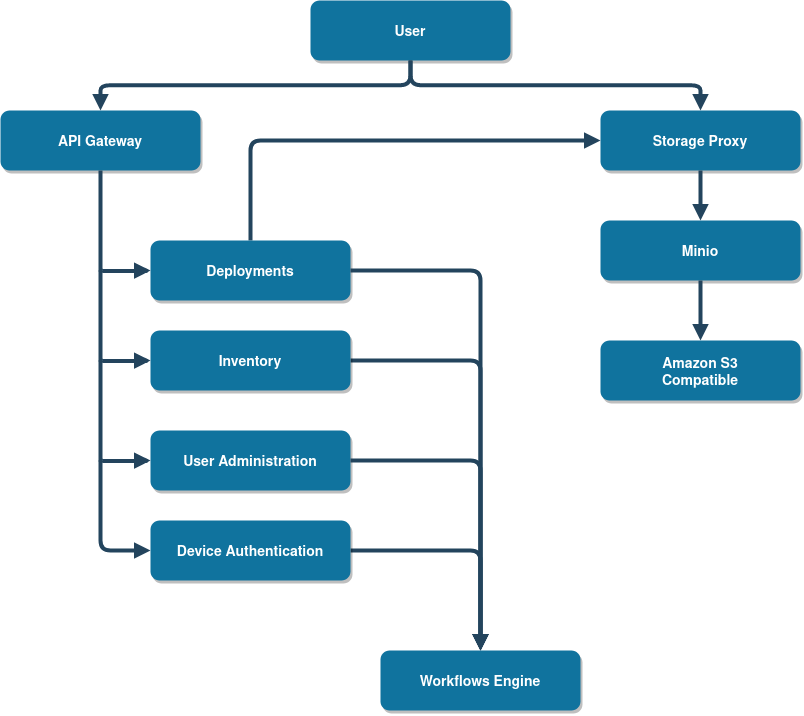
\includegraphics[scale=0.5]{images/integration-app.png}
    \caption{Mender Integration Server Architecture}
    \label{fig:mender-integration}
\end{figure}
Minio is a third-party object storage. It can either be used to serve uploaded content on its own or to proxy requests to Amazon S3 compatible cloud providers. All other services are mender application logic web services.
\newpage

\begin{code}
  \captionof{listing}{Original Docker-Compose YAML}
  \label{org-dc}
  \begin{minted}{yaml}
version: '2.1'
services:

  mender-deployments:
    command: server --automigrate
    image: mendersoftware/deployments:mender-2.4.0
    restart: on-failure
    volumes:
      - ./storage.crt:/etc/ssl/certs/storage-proxy.crt
    environment:
      STORAGE_BACKEND_CERT: /etc/ssl/certs/storage-proxy.crt
      DEPLOYMENTS_AWS_AUTH_KEY: minio
      DEPLOYMENTS_AWS_AUTH_SECRET: minio123
      DEPLOYMENTS_AWS_URI: https://storage-proxy:9000
    networks:
      - mender
    depends_on:
      - mender-mongo
      - storage-proxy

networks:
  mender:
  \end{minted}
\end{code}
Listing \ref{org-dc} shows a YAML configuration to run Mender Hub via Docker-Compose on a local machine.

Quellen:

hivemq:

hivemq extensions: https://www.hivemq.com/docs/hivemq/4.4/extensions/registries.html#modifiable-client-settings
client takeover: https://www.hivemq.com/blog/mqtt-essentials-part-10-alive-client-take-over/
resilience: https://www.hivemq.com/blog/are-your-mqtt-applications-resilient-enough/
mqtt stresser: https://github.com/inovex/mqtt-stresser
custom tlv fields in proxy protocol: https://www.hivemq.com/docs/hivemq/4.4/user-guide/proxy-protocol.html#custom-tlv

lwt and client takeover issue: https://github.com/eclipse/mosquitto/issues/904

envoy:

draining: https://www.envoyproxy.io/docs/envoy/latest/intro/arch_overview/operations/draining
life of a request: https://www.envoyproxy.io/docs/envoy/latest/intro/life_of_a_request
edge proxy: https://www.envoyproxy.io/docs/envoy/latest/configuration/best_practices/edge
tcp proxy and link to reference: https://www.envoyproxy.io/docs/envoy/latest/intro/arch_overview/listeners/tcp_proxy
timeouts: https://www.envoyproxy.io/docs/envoy/latest/faq/configuration/timeouts
hello world example: https://salmaan-rashid.medium.com/envoy-control-plane-hello-world-2f49b2865f29
exmaple with python: https://salmaan-rashid.medium.com/envoy-discovery-hello-world-d3e44d19603d
envoy discovery repo: https://github.com/salrashid123/envoy_discovery
go control plane: https://github.com/envoyproxy/go-control-plane
microservices resilience: https://www.getambassador.io/resources/getting-started-envoyproxy-microservices-resilience/
matt klein talk: https://www.youtube.com/watch?v=gQF23Vw0keg
per listener overhead too high: https://github.com/envoyproxy/envoy/issues/4196
istio performance: https://istio.io/latest/docs/ops/deployment/performance-and-scalability/

podcasts:
podcast service mesh or a platform: https://www.weave.works/blog/is-envoy-a-service-mesh-or-a-platform
envoy: https://kubernetespodcast.com/episode/033-envoy/
matt klein 1: https://developertea.simplecast.com/episodes/50464d4b-4071c0b8
matt klein 2: https://developertea.simplecast.com/episodes/10bb00cd-a148f095

papers:

LB survey: https://dl.acm.org/doi/10.1145/3281010

inovex:

confluence: https://confluence.inovex.de/display/ITKB/%28WIP%29+Smart+load+balancing+von+MQTT+traffic
jira: https://jira.inovex.de/browse/ST-2828
